\documentclass[a4paper]{article}
\usepackage{geometry}
 \geometry{
 a4paper,
 total={210mm,297mm},
 left=1.25in,
 right=1.25in,
 top=1.25in,
 bottom=1.25in,
 }
\usepackage{graphicx}
\usepackage{tgpagella}
\usepackage[T1]{fontenc}
\usepackage{amsmath}
\usepackage{amssymb}
\usepackage{float}
\usepackage{subcaption}
\usepackage[caption = false]{subfig}
\usepackage[utf8]{inputenc}
\newcommand{\argmax}{\operatorname{argmax}}

\begin{document}
\title{Iteratively Reweighted Algorithms for Compressive Sensing}
\author{Sasank Ch - 110070051\\
Tharun Kumar Reddy - 110070048}
\maketitle

\section{Introduction}
Compressive Sensing concept says that sparse signals can be reconstructed exactly with few measurements. Since MRI acquisition is a time consuming process, this technique comes handy in reducing the time required to acquire as well as memory required to store the data. The principle behind this is that we measure few linear combinations of original signal vector in an manner that the measurements are incoherent, which is explained later. The incoherence ensures that info about entire signal is captured in few measurements. 
\par
Let $\phi$ be a measuring matrix of size $M*N$,$x$ be a sparse vector which we seek to measure and $\phi x = b$ be the measured $M$-dimensional vector of $N$-dimensional signal $x$ where $ M<N $. The reconstructed signal $x^*$ is given by 
\begin{equation}
min_u ||u||_1 
\end{equation}

subject to  $\phi u=b$. 
\newline We ideally want to minimize $L-0$ norm rather than $L-1$ norm but former being NP-hard, we perform a softer version called Basis Pursuit.


  


\section{Theorem supporting recovery by basis pursuit}
\begin{itemize}
\item Consider a signal vector $f$ (having length $n$) with a sparse
representation in basis $\psi$, i.e. $f =  \psi \theta$ where $|\theta |<< n$. $\phi$ be $M*N$ measurement matrix as mentioned before.  If $m\geq C lon(n/\delta)K\mu^2(\psi,\phi)$ (C is some constant) then the solution to the Compressive Sensing problem is exact with probability $1-\delta$
\end{itemize}

\noindent Here, $K$ denoted $L-0$ norm aka sparsity of $x$. C depends on $\delta$ but tends to 1 as $N$ tends to $\infty$. $\phi$ can be any of a random fourier submatrix, random Gaussian matrix with mean zero and columns normalized or random Bernoulli matrix with columns normalized etc. All these constructions are incoherent with any orthonormal basis. 
\section{Iteratively Reweighted Least Squares(IRLS) Algorithm}
The approach is to
replace the $l^p$ objective function in (1) by a weighted $l^2$ norm
\begin{equation}
min_u \sum_i w_i u_i^2 
\end{equation}

subject to  $\phi u=b$.
\newline Th weights are iteratively computed so as to approximate in first order sense the $l^p$ objective, given by $w_i=|{u_i}^{(n-1)}|^{p-2}$ . The solution to to (2) is then explicitly given by 
\begin{equation}
u^{(n)}=Q_n\phi^T(\phi Q_n \phi^T)^{-1}b
\end{equation}
where $Q_n$ is the diagonal matrix with entries $1/w_i$. To overcome the case where $w_i$ shoots up due to $u_i$ being zero, we use damping approach as follows
\begin{equation}
w_i=(({u_i}^{(n-1)})^2+\epsilon)^{p/2 - 1}
\end{equation} 

\section{IRL1 variant of previous algorithm}
The entire approach remains same except for the objective function being 
\begin{equation}
min_u \sum_i w_i |u_i| 
\end{equation}

subject to  $\phi u=b$. The weights are given by 
\begin{equation}
w_i=(|{u_i}^{(n-1)}|+\epsilon)^{p - 1}
\end{equation} 


\section{Dataset}
We used the Cardiac MRI dataset from York University to test our implementation. The dataset consisted of 7098(of size 256*256 each) images of 33 persons in various orientations. We randomly chose  one image per person (total 33 images). Since the data was given as images, we represented the data in sparse basis like Fourier and DCT for our experiments. 
\par We are ideally supposed to reshape the images to 65526*1 images and acquire combinations of sparse data. But here, size of $\phi$ and    $Q_n$ is so huge and not supported by MATLAB. Hence, we preferred to reconstruct each 256*1 column separately to yield a whole image.



\section{Implementation}
\begin{itemize}
\item For each image, we first calculated the sparse representation in DCT basis.
\item We chose $\phi$ to be random bernouli matrix with p=0.5(symmetric) and normalized the columns.
\item Then, we calculated $b=\phi u$.
\item We then initialized $u^{(0)}$ to minimum $l^2$ norm solution, i.e . psuedo inverse solution. 
\item Performed the iterations varying p among 0,1 and algorithm among IRLS and IRL1
\end{itemize}
     
\section{Results}
For 2/3 compression, Figure 1 and 2 show some of the good and bad reconstructions. For 1/2 compression, Figure 3 and 4 show some of the good and bad reconstructions.


\begin{figure}[h]
\begin{subfigure}{.5\textwidth}
  \centering
  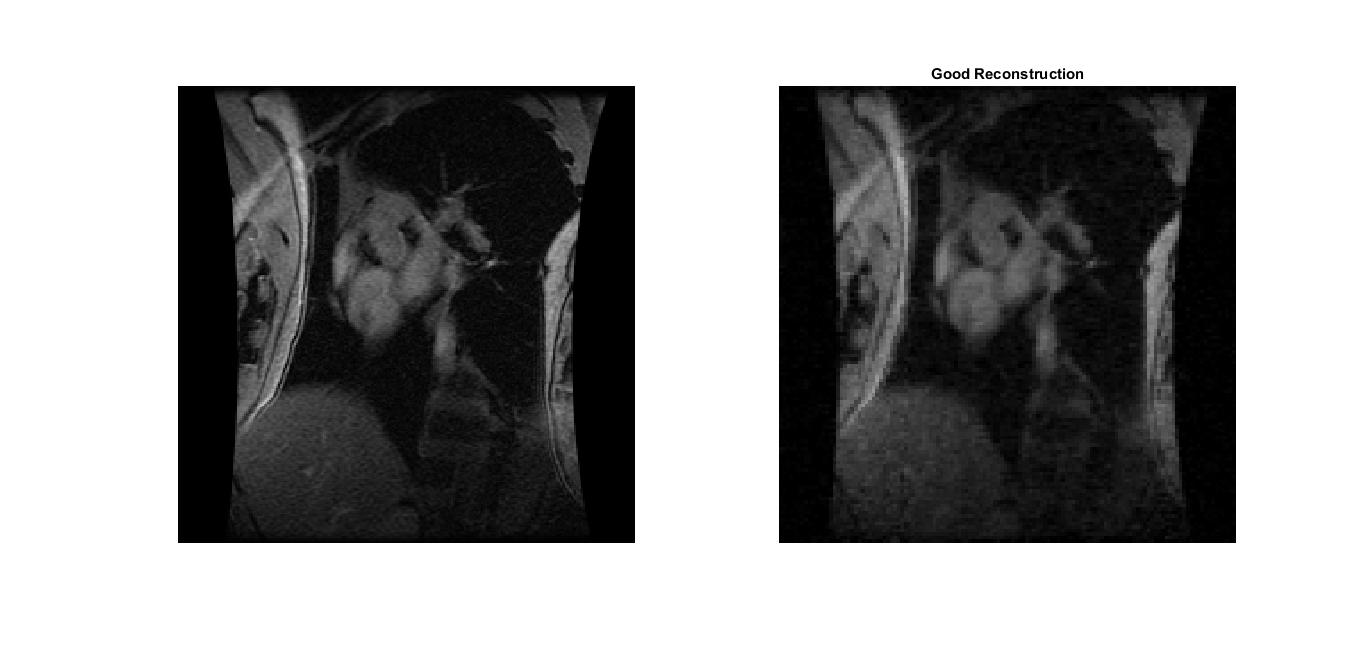
\includegraphics[width = 6in]{good11.jpg}
  \label{fig:sfig1}
\end{subfigure}%

\begin{subfigure}{.5\textwidth}
  \centering
  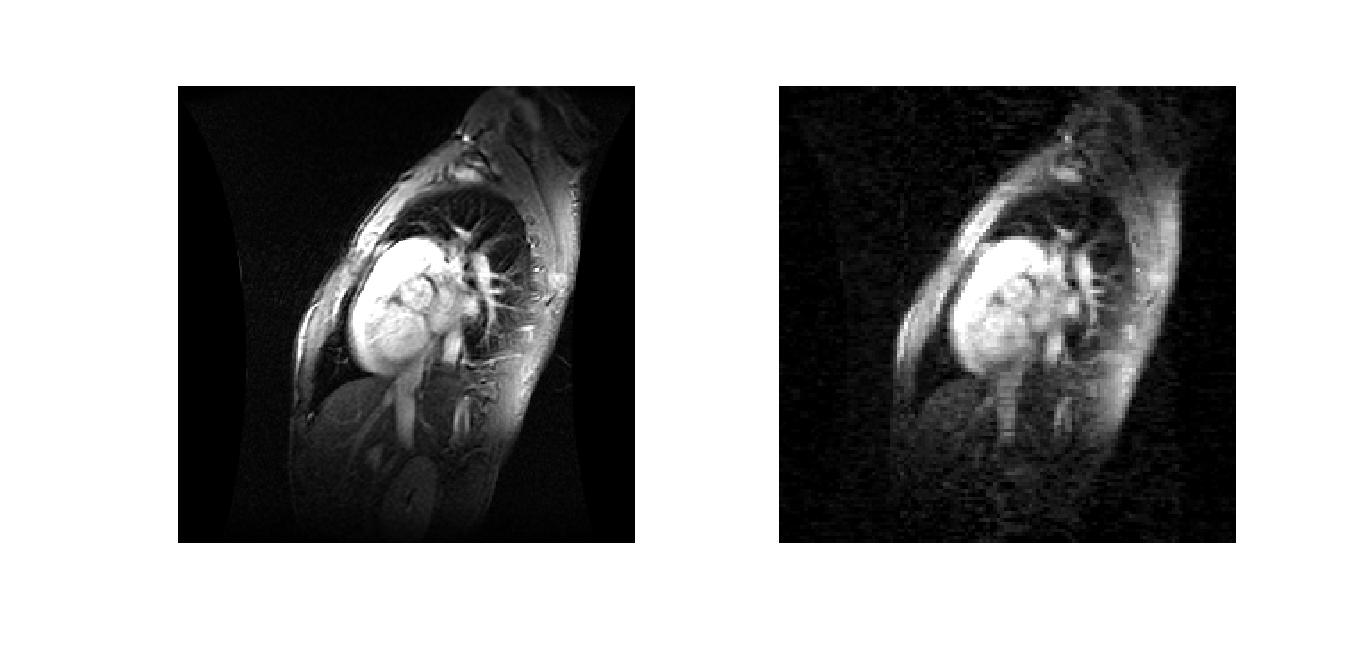
\includegraphics[width = 6in]{good12.jpg}
  \label{fig:sfig2}
\end{subfigure}

\begin{subfigure}{.5\textwidth}
  \centering
  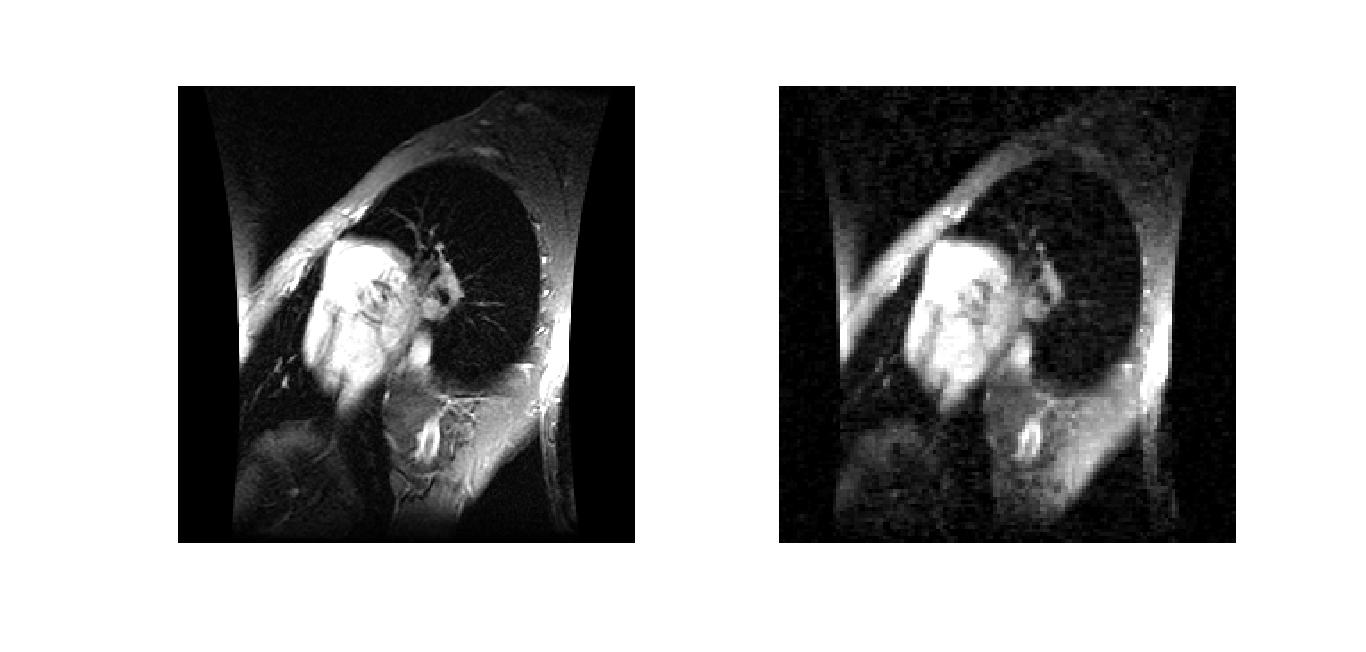
\includegraphics[width = 6in]{good13.jpg}
  \label{fig:sfig2}
\end{subfigure}
\caption{Good Reconstructions for 2/3 Compression}
\end{figure}

\begin{figure}[h]
\begin{subfigure}{.5\textwidth}
  \centering
  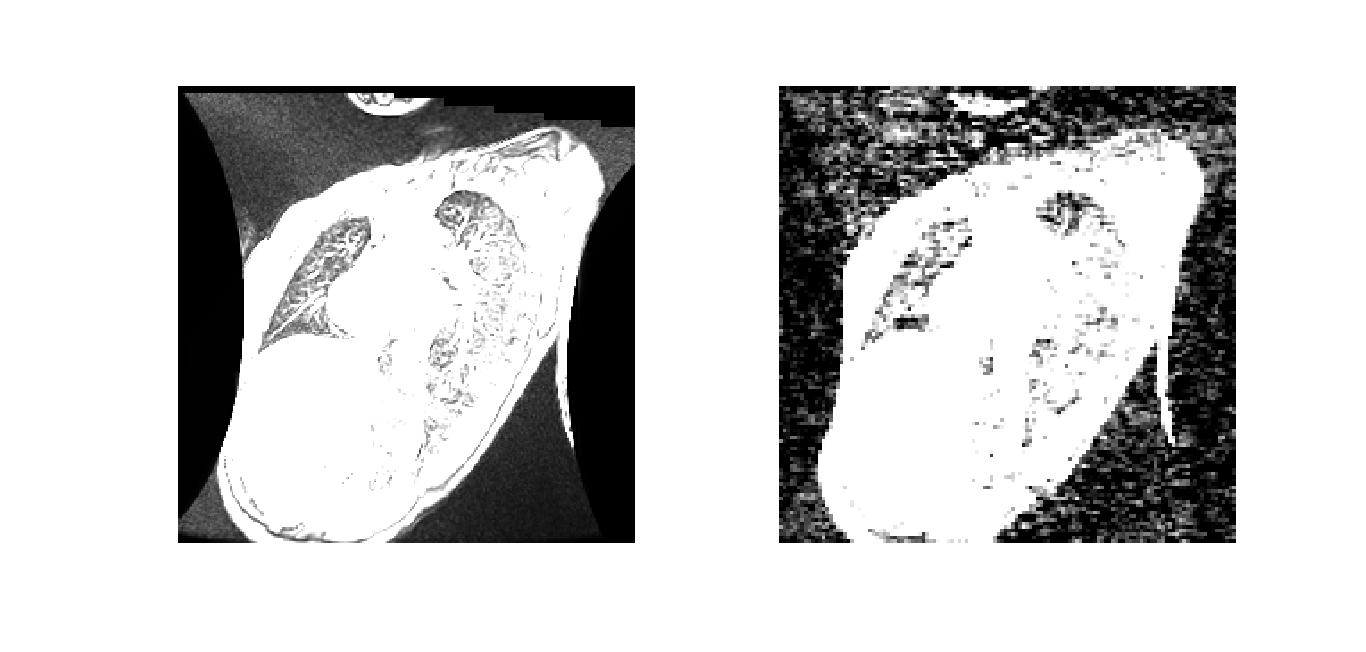
\includegraphics[width = 6in]{bad11.jpg}
  \label{fig:sfig1}
\end{subfigure}%

\begin{subfigure}{.5\textwidth}
  \centering
  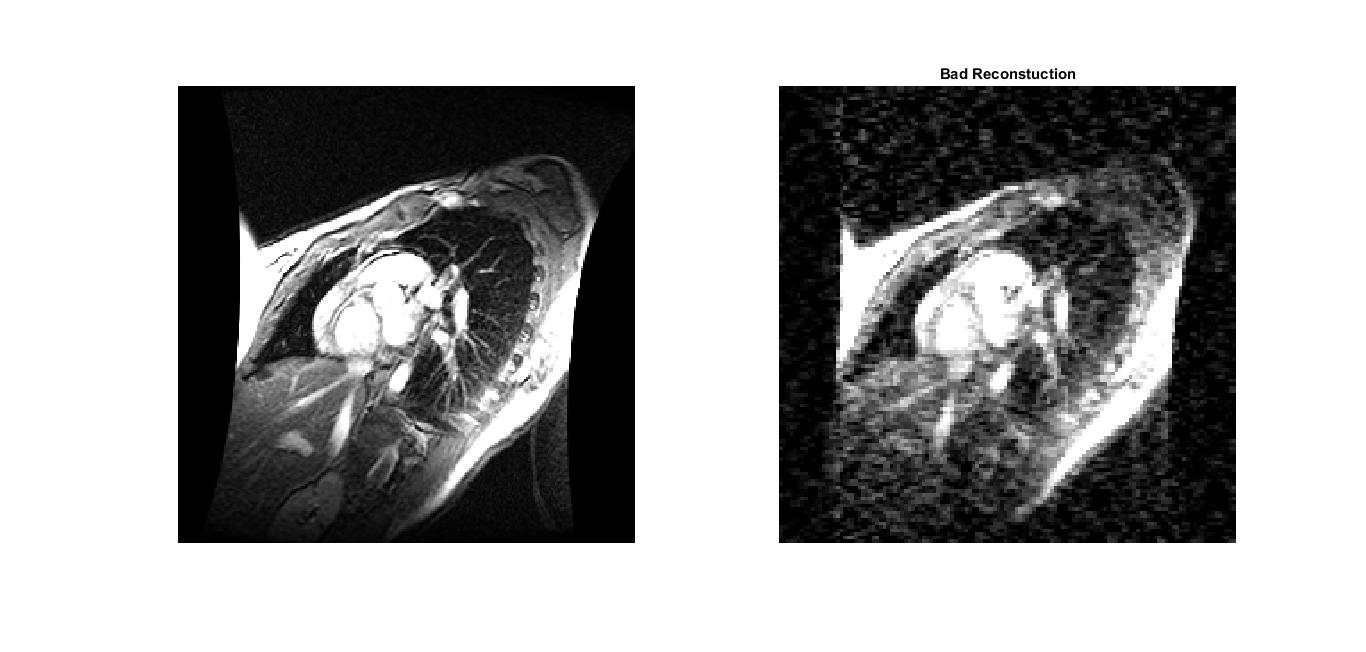
\includegraphics[width = 6in]{bad12.jpg}
  \label{fig:sfig2}
\end{subfigure}
\caption{Bad Reconstructions for 2/3 Compression}
\end{figure}


\begin{figure}[h]
\begin{subfigure}{.5\textwidth}
  \centering
  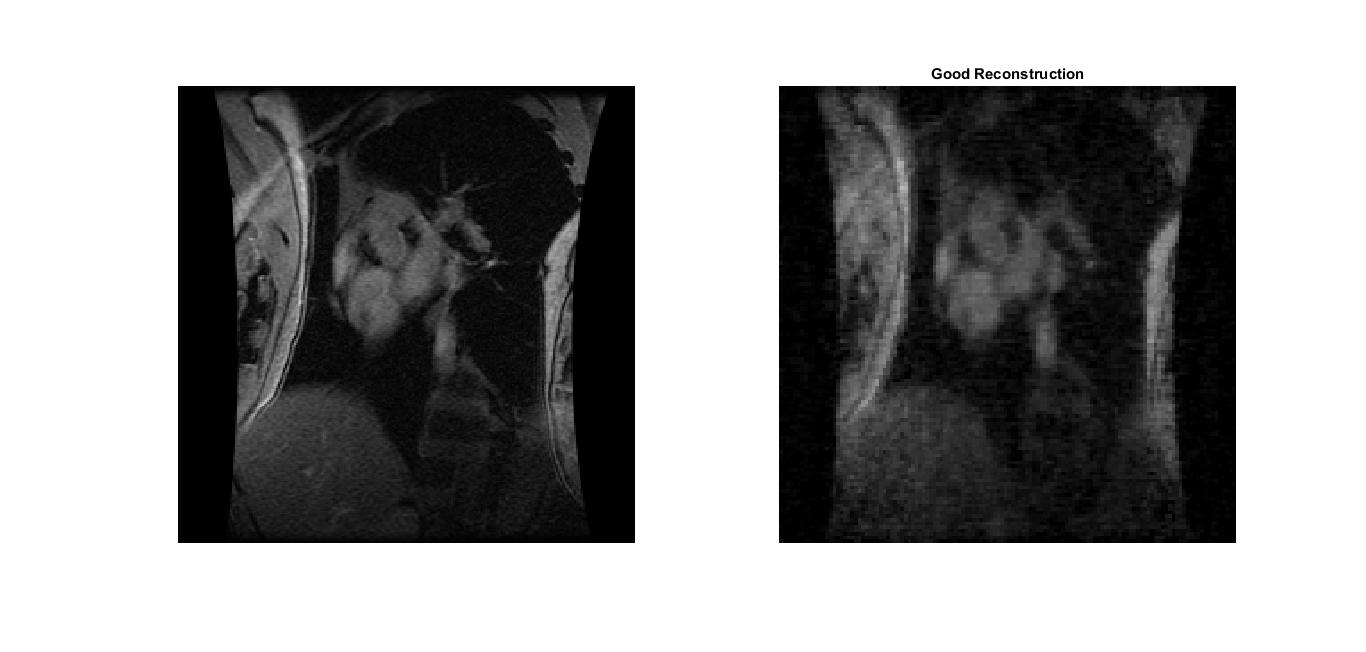
\includegraphics[width = 6in]{good21.jpg}
  \label{fig:sfig1}
\end{subfigure}%

\begin{subfigure}{.5\textwidth}
  \centering
  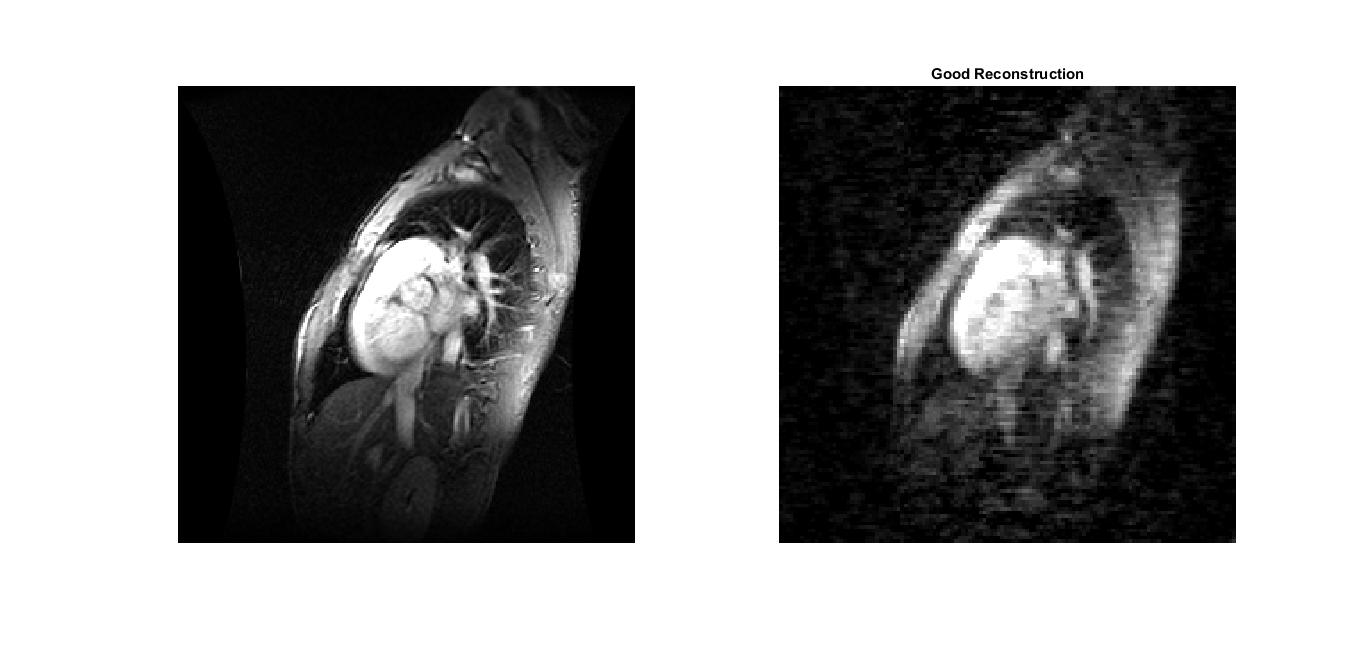
\includegraphics[width = 6in]{good22.jpg}
  \label{fig:sfig2}
\end{subfigure}

\begin{subfigure}{.5\textwidth}
  \centering
  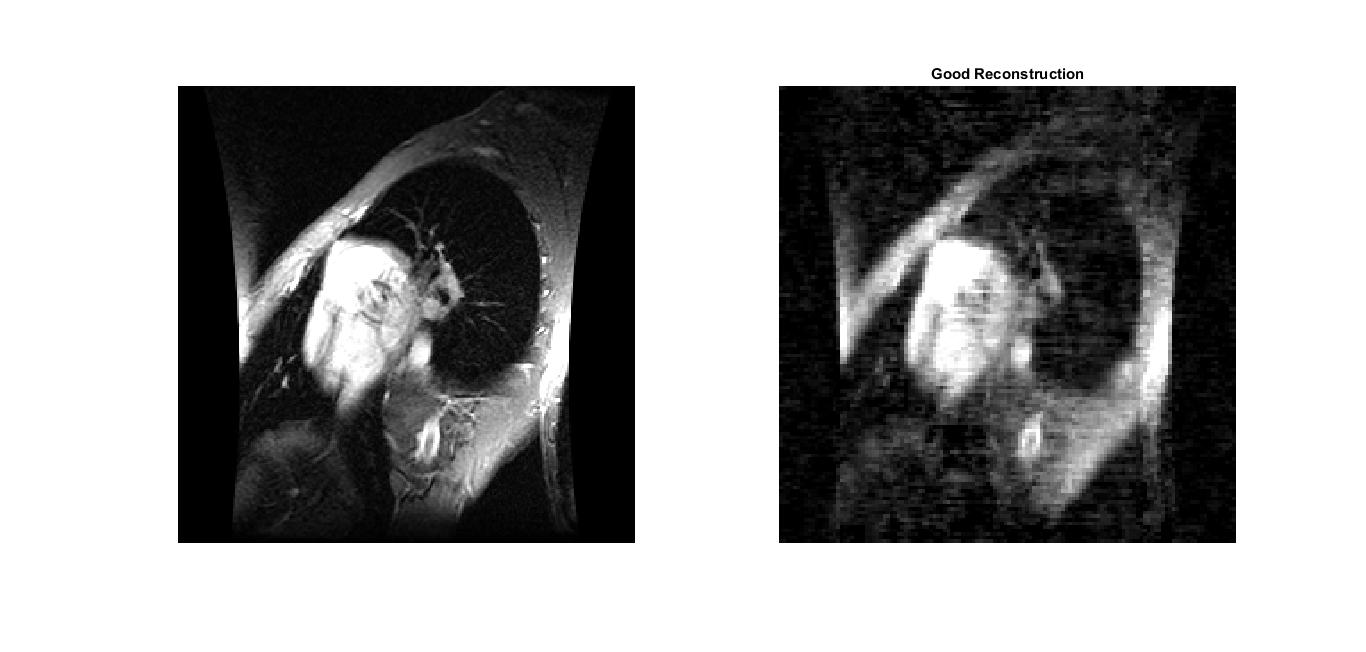
\includegraphics[width = 6in]{good23.jpg}
  \label{fig:sfig2}
\end{subfigure}
\caption{Good Reconstructions for 1/2 Compression}
\end{figure}

\begin{figure}[h]
\begin{subfigure}{.5\textwidth}
  \centering
  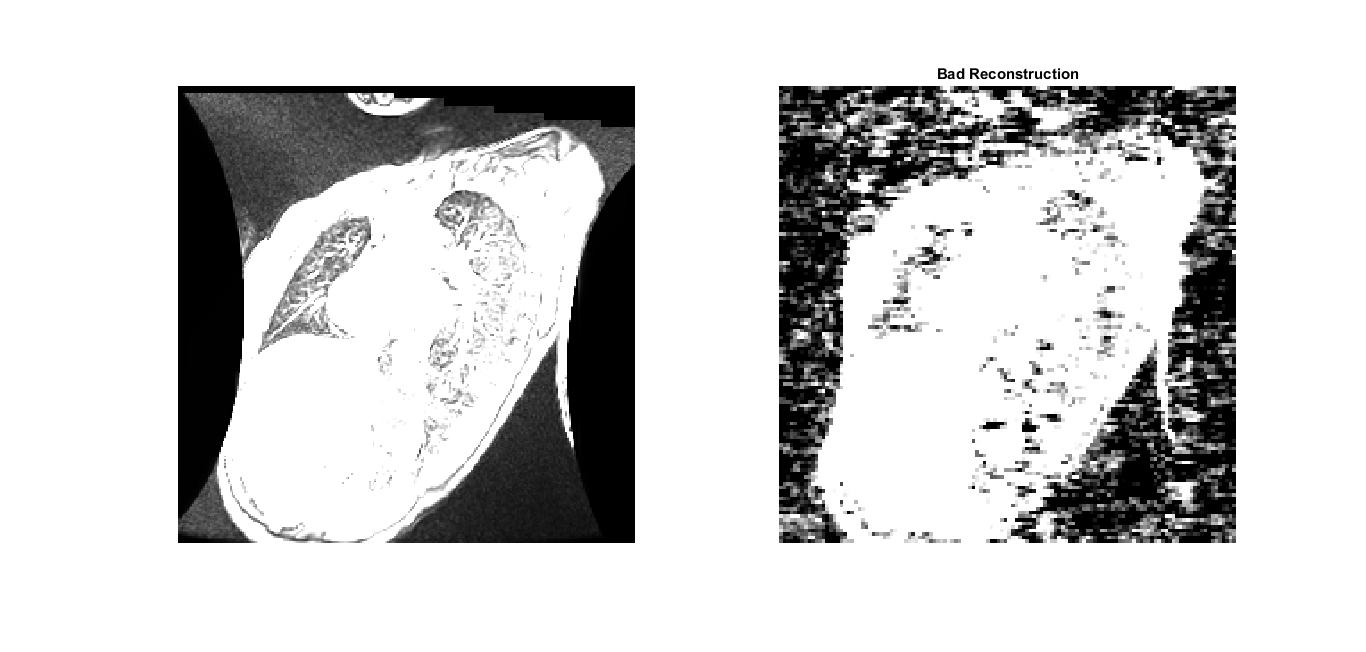
\includegraphics[width = 6in]{bad21.jpg}
  \label{fig:sfig1}
\end{subfigure}%

\begin{subfigure}{.5\textwidth}
  \centering
  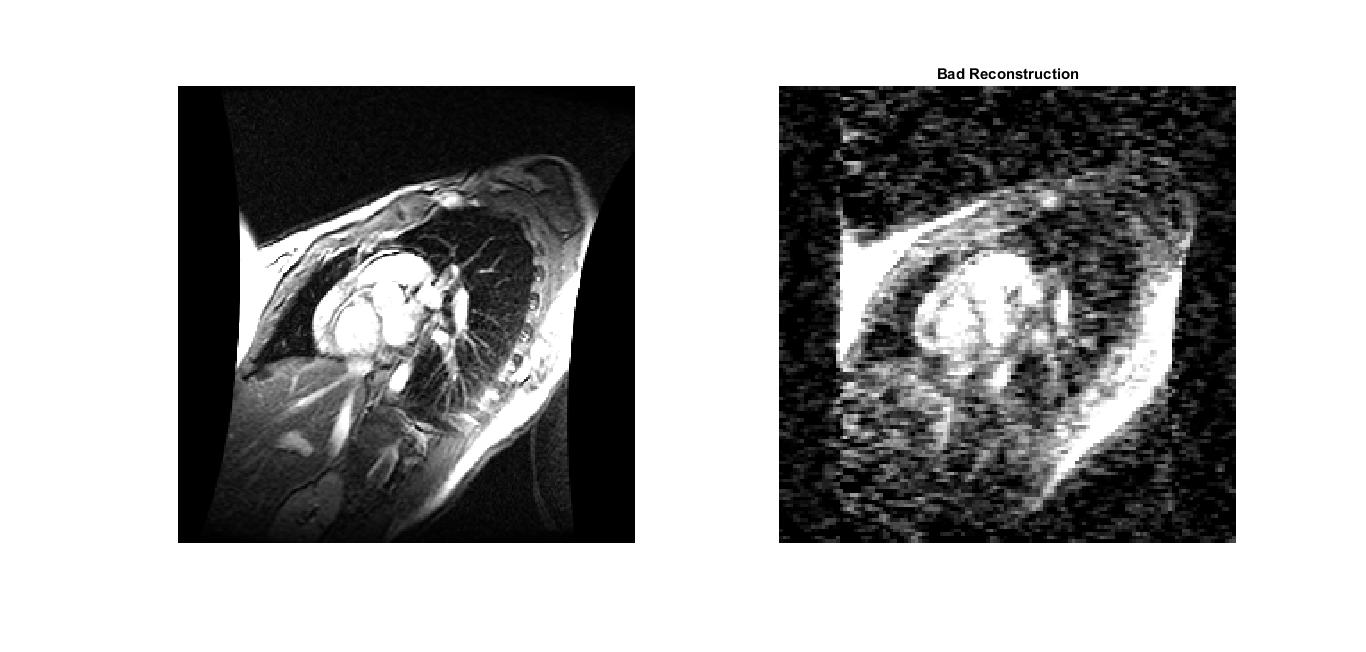
\includegraphics[width = 6in]{bad22.jpg}
  \label{fig:sfig2}
\end{subfigure}
\caption{Bad Reconstructions for 1/2 Compression}
\end{figure}

\begin{figure}
\centering
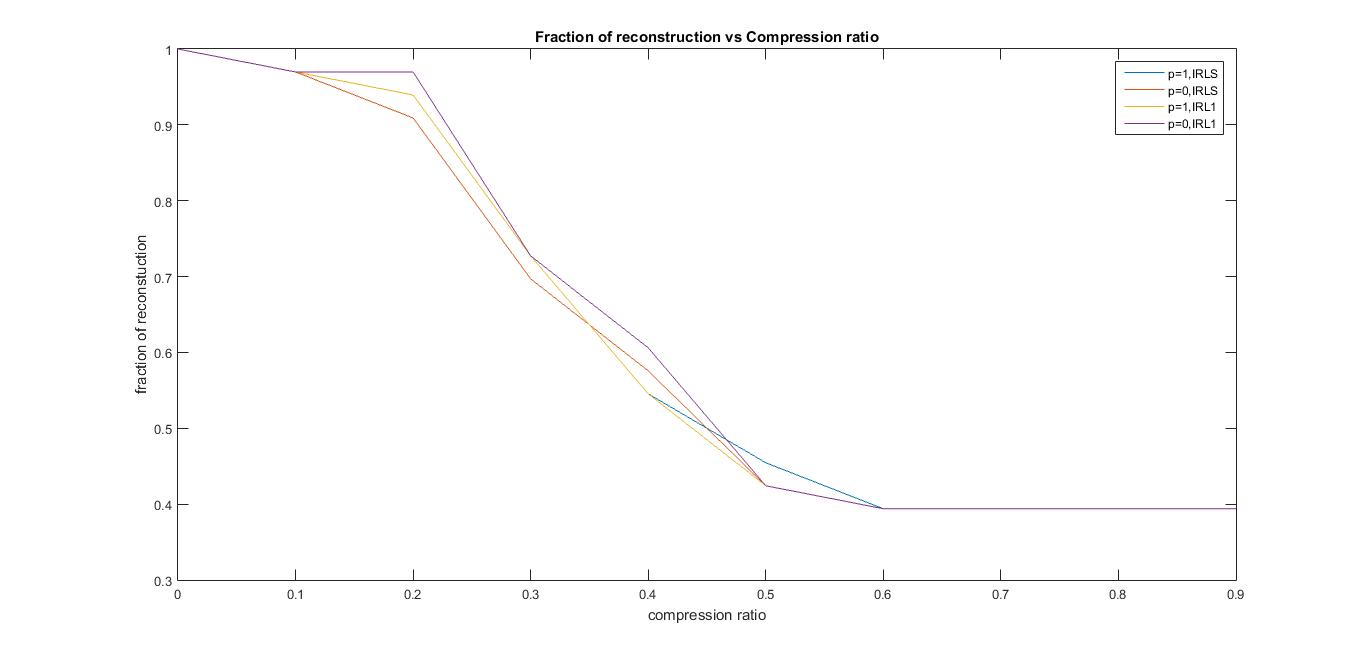
\includegraphics[width = 7in]{combo3.jpg}
\caption{Reconstruction vs Compression}
\end{figure}
\end{document}
